\chapter{Dicas}

Dicas de uso de citação, equações, figuras e tabelas

\subsection{Citação}
Lembre de adicionar as referências no arquivo .bib

Citação direta... Segundo \cite{accardi2012}.

Citação indireta... \citep{accardi2012}

\subsection{Equações}

Dê uma olhada no arquivo macros.tex e adicione o que tiver interesse. Lembre sempre de referenciar equações numeradas. (...) como pode ser visto na Equação \ref{eq:teste}.

\begin{equation}
    \stateStart = \begin{bmatrix}
        \cos{\phi} & \sin{\phi} & 0
    \end{bmatrix}^\top \in \set{\Omega} \subset \R^3
    \label{eq:teste}
\end{equation}

Também é possível montar uma equação multilinha, como pode ser visto em \ref{eq:problem_mpc}.
\begin{equation}
    \begin{split}
        \text{minimizar} & \quad \sum_{k = 0}^{k = N} (\stateVec(k) - \refVec(k))^\top \matr{Q}(k) (\stateVec(k) - \refVec(k)) + \sum_{k = 0}^{k = N - 1} \inputVec(k)^\top \matr{R}(k) \inputVec(k), \\
        \text{sujeita a} & \quad \stateVec(k+1) = \matr{F} \stateVec(k) + \matr{G} \inputVec(k), \\
        & \quad \stateVec_{\min} \leq \stateVec(k)\leq \stateVec_{\max}, \\
        & \quad \inputVec_{\min} \leq \inputVec(k)\leq \inputVec_{\max}, \\
        & \quad \stateVec(0) = \stateVec_0.
    \end{split}
    \label{eq:problem_mpc}
\end{equation}

\subsection{Figuras}

Lembre de sempre referenciar figuras. (...) Como pode ser visto na Figura \ref{fig:imagemEstande}.

\begin{figure}[H]
    \centering
    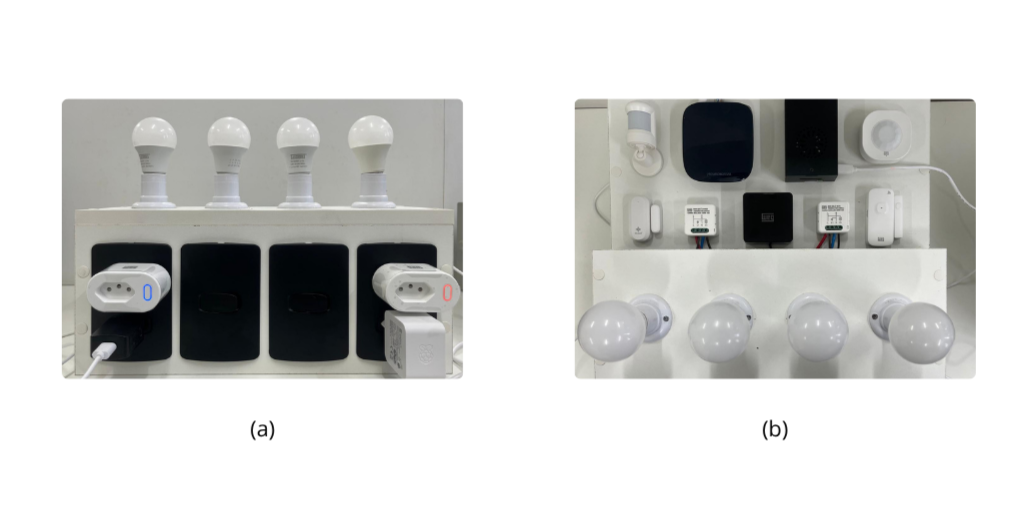
\includegraphics[width=\linewidth]{Cap03/img/vistaEstande.png}
    \caption{Fotos do Estande desenvolvido para aplicação: (a)Vista Frontal - Disposição de tomadas, tomadas inteligentes e interruptores; (b) Vista Superior - Disposição das lâmpadas, sensores, atuadores e controladores.}
    \label{fig:imagemEstande}
\end{figure}

\subsection{Tabela}

Lembre de sempre referenciar tabelas. (...) Como pode ser visto na Tabel \ref{tab:devices}.

\newcolumntype{P}[1]{>{\centering\arraybackslash}p{#1}}
\begin{table}[h]
    \centering
    \renewcommand{\arraystretch}{1.5} % aumenta altura das linhas
    \begin{tabular}{P{4cm}P{2cm}P{2.8cm}P{5cm}}
        \hline
        \textbf{Dispositivo} & \textbf{Protocolo} & \textbf{Marca} & \textbf{Função} \\
        \hline
        Roteador Wi-Fi & Wi-Fi & Tp-Link & Roteamento da rede e conexão com a internet \\
        Hub Zigbee & Zigbee & Nova Digital & Coordenador da rede Zigbee\\
        Sensor de Porta & Wi-Fi & WEG & Detecção de abertura/fechamento \\
        Sensor de Movimento & Wi-Fi & WEG & Detecção de movimento \\
        Sensor de Porta & Zigbee & Ekasa & Detecção de abertura/fechamento \\
        Sensor de Movimento & Zigbee & Nova Digital & Detecção de movimento \\
        Relé inteligente & Wi-Fi & WEG & Controle de carga via Wi-Fi \\
        Tomada inteligente & Wi-Fi & WEG & Acionamento remoto de equipamentos\\
        Relé inteligente & Zigbee & WEG & Controle de carga via Zigbee \\
        Tomada inteligente & Zigbee & WEG & Acionamento remoto de equipamentos\\
        Central de Automação & - & Raspberry Pi 5 & Execução do Home Assistant \\
        \hline
    \end{tabular}
    \caption{Lista de dispositivos do estande}
    \label{tab:devices}
\end{table}
